\RequirePackage[T1]{fontenc}
\documentclass[conference]{IEEEtran}
\usepackage{cite}
\usepackage{amsmath}
\usepackage{graphicx}
\usepackage{booktabs}
\usepackage{array}
\usepackage[hidelinks,pdfversion=1.7]{hyperref}
\hypersetup{pdftitle={Persona-Aware, Knowledge-Bounded NPC Dialogue Through Model-Agnostic LLM Orchestration},pdfauthor={Mohan Chandra S S, Shreyas C, Nithish Gowda H N, Nithin S}}
\begin{document}
\title{Persona-Aware, Knowledge-Bounded NPC Dialogue Through Model-Agnostic LLM Orchestration}
\author{\IEEEauthorblockN{Mohan Chandra S S, Shreyas C, Nithish Gowda H N, Nithin S}
\IEEEauthorblockA{RV University\\USNs (in author order): 1RVU23CSE282, 1RVU23CSE443, 1RVU23CSE317, 1RVU23CSE316}}
\maketitle
\begin{abstract}
Language models let non-player characters (NPCs) hold open conversations, but a model connected directly to a game answers from its own knowledge and breaks character: a peasant asked for the king's war plan should not know it. Training a custom model per game is costly and ties world knowledge to model weights. We propose a generalized orchestration layer between game and model that decides whether an NPC engages, what it may know and how it responds before any model is called. World knowledge comes from creator documents through scoped retrieval, so no training is needed, while thin connectors and a one-method provider contract isolate game and model. We implemented the layer as Anima, with a Skyrim connector and an optional vision path. In a two-world study, restricted facts reached a lower-standing NPC's prompt in 75 of 80 turns without scoping and 0 of 80 with it. Scripted tests confirmed rule conformance and safe fault handling. Hosted-model and live-game samples show the boundary working, with unsupported details and fallback replies. Vision changed no decision in 66 test pairs, and a capture fix cut black pixels from 98.8\% (median) to 6.2\%. Accuracy, a second game and human ratings remain open.
\end{abstract}
\begin{IEEEkeywords}
non-player characters, large language models, orchestration, retrieval-augmented generation, computer vision, knowledge boundaries, game AI
\end{IEEEkeywords}

\section{Introduction}
Scripted dialogue cannot handle what writers did not anticipate, while language models raise problems of control~\cite{gallotta2024}. A model connected directly to an NPC brings its own general knowledge and helpfulness, so characters answer things they could not know. Consider a peasant asked for the king's war plan. The peasant has never met the king and should not know the plan, though may repeat a rumour. The king's adviser, asked the same question, does know it. Replies must follow from an NPC's standing in the world, so that the character seems to live there. We call this aim believable and make no claim of sentience.

Two practical barriers stand in the way. Training a character model for each game is expensive and fixes world knowledge in its weights~\cite{shao2023,hu2022}. Connecting to games is also hard to generalize, because each exposes different data through its mod support, and mods such as Mantella~\cite{mantella} are tied to specific titles.

We therefore propose an orchestration layer with common contracts, thin game connectors and a replaceable model. A creator supplies documents instead of training a model, retrieval~\cite{lewis2020} provides them at inference time, and deterministic rules decide behaviour before any model call. Our contributions are a layered architecture implemented with a working Skyrim connector; per-NPC knowledge binding and a deterministic conversation director applied before generation; a trust boundary for camera-derived scene descriptions; and an evaluation of knowledge boundaries, fault handling, model independence and live delivery.

\section{Related Work}
Persona-Chat established profile-conditioned dialogue~\cite{zhang2018}. Character-LLM and RoleLLM adapt model parameters to characters~\cite{shao2023,wang2024}, and LoRA lowers that cost~\cite{hu2022}, but knowledge changes then need new training. TimeChara shows strong models revealing what a character should not yet know~\cite{ahn2024}, and RoleFact attributes this to built-in knowledge~\cite{sadeq2024}.

RAG supplies knowledge at inference time~\cite{lewis2020,karpukhin2020}. RAGAs separates relevance from faithfulness~\cite{es2024}, and long contexts are not reliably used~\cite{liu2024}. Generative Agents combines memory, retrieval and planning~\cite{park2023}, and tabletop research examines game-state tracking in dialogue~\cite{callison2022}.

For vision, YOLO provides real-time detection~\cite{redmon2016}, though general-object classes do not cover game-specific entities. CLIP links images and language in a shared embedding space~\cite{radford2021}, and vision-language models such as Qwen2.5-VL return structured descriptions directly~\cite{bai2025}. Rade\v{z} and Bohak ground NPC dialogue in panoramic images and segmentation~\cite{radez2026}.

These components are established. What we add is their composition as a reusable runtime layer that applies engagement decisions and per-NPC knowledge limits before generation, without training, and that treats a camera frame as what the player sees rather than what the NPC perceives.

\section{Problem Formulation and Research Contributions}
For NPC $n$, the input is utterance $u$, trusted game state $s$, persona $p$, completed history $H$, conversation state $C$ and documents $D$, of which only a bound subset $D_n$ is available. The task is constrained dialogue generation: output a validated reply $y$, or decide not to generate.
\begin{align}
c&=A(u,s,p,H), & a&=\pi(c),\nonumber\\
m_0&=M(u,C,p), & E&=R(q,D_n,k),\nonumber\\
m&=F(m_0,E,C), & y&=G(B(c,a,m,E)).\nonumber
\end{align}
Here $A$ appraises the situation, $\pi$ selects a route, $M$ selects a conversational move, $R$ returns at most $k=3$ passages for query $q$, $F$ revises the move once material is known, $B$ builds the prompt, and $G$ is any model. Acceptance check $V$ decides whether $y$ leaves the layer. Authored and end routes skip $R$ and $G$. Since $G$ may still add facts from its own weights, the bound covers supplied context only.

We ask: \textbf{RQ1}, does binding keep restricted knowledge from NPCs that should not have it, and with what real-model behaviour? \textbf{RQ2}, does the layer hold when the model fails or the player applies pressure? \textbf{RQ3}, what must change for a new model or world? \textbf{RQ4}, do replies reach a real game and enter memory? \textbf{RQ5}, what can computer vision add, and does its trust boundary hold?

\section{Proposed System Architecture}
Fig.~\ref{fig:architecture} shows the layers. The \textbf{core} holds no game or vendor logic and composes each turn: appraisal keeps only facts the NPC could perceive, policy selects a route, the director selects a move, retrieval fetches bound evidence, and validation accepts or rejects the reply. \textbf{Knowledge} is prepared offline from creator files. \textbf{Models} sit behind one interface. The \textbf{connector} maps a game's data to the contracts, loads social state, delivers replies and returns receipts, and only completed turns enter memory.

\begin{figure*}[t]
\centering
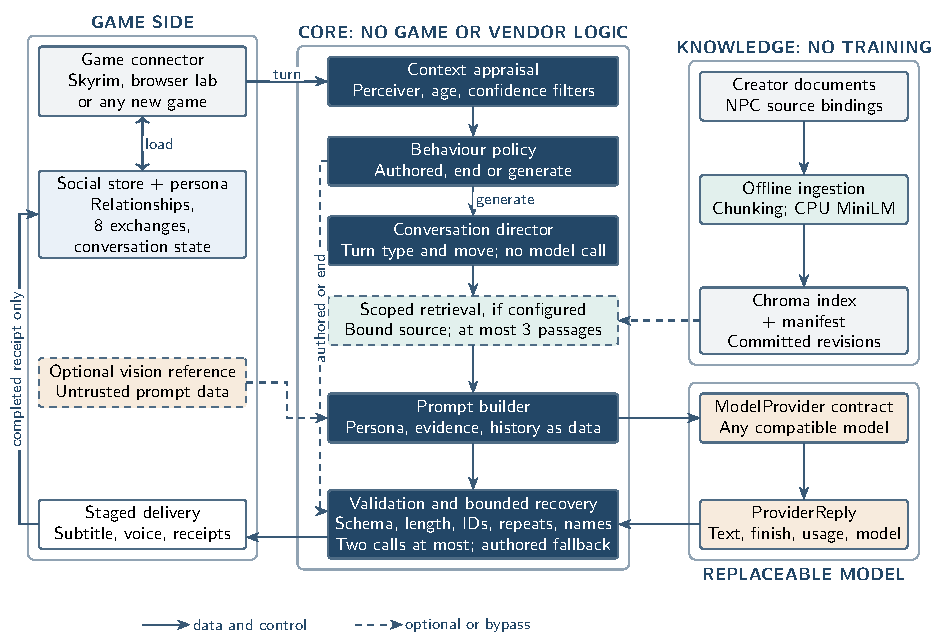
\includegraphics[width=.8\textwidth]{figures/system_architecture.pdf}
\caption{Proposed architecture. Only the connector knows the game, and only the provider contract knows the model. Dashed elements are optional or bypass paths.}
\label{fig:architecture}
\end{figure*}

\textit{What a new game supplies.} A connector provides player text or speech; stable NPC and player identifiers; world and save scope; location, time, combat and availability state; and facts with source, age, confidence and perceivers. It shows only validated text, honours expiry, stops on interruption or combat, and reports started, completed, interrupted or failed receipts. Model output cannot change game state. Creators add personas and documents, and a missing fact stays unknown rather than being invented. Thin connectors built on existing mod support are the intended route, since a universal connector is impractical. Generality across games remains a design goal, because one game is connected so far.

\section{System Methodology}
\subsection{Scoped Knowledge Without Training}
Loaders read plain-text, structured, PDF, DOCX and HTML files. Text becomes 220-token chunks with 32-token overlap, embedded by all-MiniLM-L6-v2~\cite{minilm2020,minilm_model} on CPU through ONNX Runtime~\cite{onnxruntime} and stored in Chroma~\cite{chroma} with source and revision metadata. Changing what an NPC knows means editing a file and re-indexing. A trusted configuration binds each NPC to one source file. Filtering precedes ranking, so similarity cannot grant access (Fig.~\ref{fig:binding}), and each hit is rechecked afterwards. Up to eight candidates are retrieved so that passages already told can be removed, and at most three reach the prompt. Layered public, regional and faction sources are not yet implemented.

\begin{figure}[t]
\centering
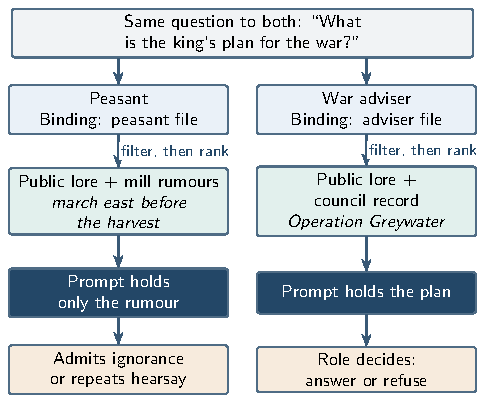
\includegraphics[width=.94\columnwidth]{figures/knowledge_binding.pdf}
\caption{Knowledge binding. One question, one engine, different knowledge, because each NPC can read only its bound source.}
\label{fig:binding}
\end{figure}

\subsection{Dialogue Turn and Conversation Director}
Fig.~\ref{fig:workflow} traces one turn. Hard rules for combat, threats, insults, availability and greetings run first, with authored lines that need no model. Across four identical questions, an earlier build sent byte-identical instructions and limits, so NPCs repeated themselves. The director fixes this without a model call. It reads a turn as new, repeat, rephrase, follow-up, push-back, shared news, stall, answered or return, then chooses a move such as answer, expand, answer differently, challenge, close topic, hold, admit limit or react. The move, a conversation brief, phrases to avoid and items already told enter the prompt. Rapport affects length and warmth only, and repetition never changes knowledge access or trust.

\begin{figure}[t]
\centering
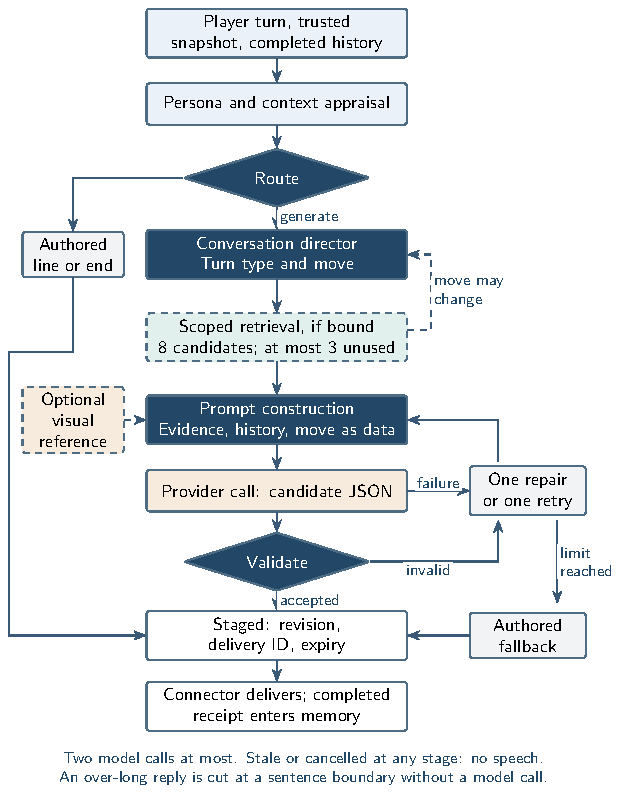
\includegraphics[width=.98\columnwidth]{figures/rag_orchestration_pipeline.pdf}
\caption{Workflow for one dialogue turn. A retrieval result can revise the move, for example to admit limit when nothing new remains.}
\label{fig:workflow}
\end{figure}

\subsection{Model Boundary and Acceptance}
Prompts are structured and zero-shot. System content holds identity, goals, boundaries and limits, and permits in-character opinion and labelled hearsay while barring invented specifics. Player text, passages, history and visual descriptions are labelled as untrusted data, which is a prompt boundary and no proven injection defence. A model is reached through one method, \texttt{ModelProvider.generate} (Fig.~\ref{fig:provider}), so a compatible endpoint needs only a profile and another protocol needs one new class.

The validator enforces strict JSON, length, modes, cues and supplied citations, and rejects assistant-style phrasing, repeated replies and capitalized names absent from the context. It does not verify claims against evidence. Recovery allows one repair or one transient retry, then an authored fallback, with at most two model calls. Rate-limit and authentication errors are not retried. Stale or cancelled work produces no speech.

\begin{figure}[t]
\centering
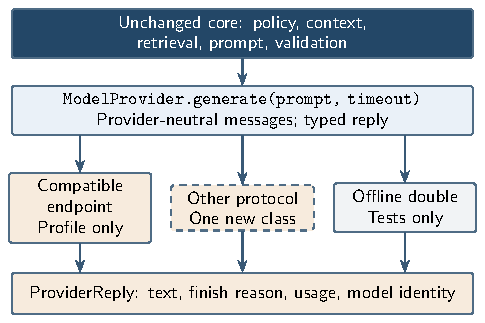
\includegraphics[width=.92\columnwidth]{figures/model_agnostic_architecture.pdf}
\caption{Provider boundary. Backends change by configuration; other protocols need an adapter.}
\label{fig:provider}
\end{figure}

\subsection{Visual Context From the Player's View}
Games report only part of what is happening, so a camera frame is the one context source that does not depend on mod support. Fig.~\ref{fig:cv} shows the optional path. To avoid continuous inference beside the game, frames are taken when a conversation opens or context changes materially, plus on a player turn when CV is on and no fresh description exists. A local vision-language model~\cite{bai2025}, through Ollama at temperature zero, returns JSON that is validated into a versioned scene descriptor. Non-conforming objects are rejected, while minor type mismatches are coerced. A YOLO detector~\cite{redmon2016} is retained but disabled, since it adds a second GPU stack and cannot identify game-specific entities.

\begin{figure}[t]
\centering
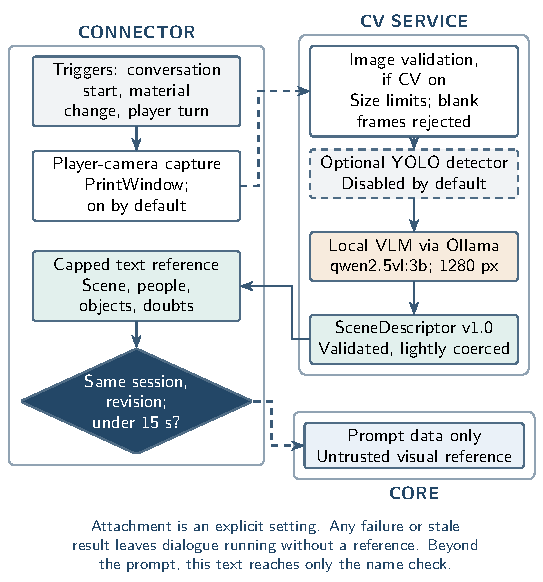
\includegraphics[width=.94\columnwidth]{figures/cv_scene_pipeline.pdf}
\caption{Optional vision path, grouped by process. A frame becomes a capped, expiring, untrusted text reference.}
\label{fig:cv}
\end{figure}

The camera shows what the player sees, which is not what the NPC sees. The result is therefore cut to one environment line, four characters, eight objects and four uncertainties, bound to session and revision, and expired after 15~s. It enters the prompt only as an untrusted reference. It cannot change route, move, trust, retrieval or memory, and it cannot be cited. CV analysis and prompt attachment are off by default, while screenshot capture itself is on.

\section{Implementation and Experimental Setup}
The system runs locally on an Intel Core i7-13700HX with Windows, Python 3.11.9 and Skyrim SE 1.7.104, using a hosted model. The Skyrim connector pairs a native SKSE plugin with a loopback Python bridge and does not call Mantella code. It accepts typed text and held-key speech through faster-whisper on CPU. It speaks through Piper voices played on system audio, so voice is not positional, with subtitles timed to the planned duration. Unauthored NPCs receive default personas from role rules. A live profile cuts off a model call after 4~s and retries a transient failure once. The full offline regression suite, of over 900 tests, passed at the time of writing.

We report five studies and do not pool them. \textbf{S1, knowledge scope:} two authored worlds, a kingdom and a space station, with three roles each at different standing and 120 fixed turns per condition, including direct, paraphrased, false-authority and injection queries. The real pipeline runs with a recording stub. The unscoped baseline merges all files into one index; the scoped condition binds each NPC to its own file. Marker phrases fixed in advance detect restricted facts in the provider-bound prompt. \textbf{S2, orchestration:} the real pipeline with scripted models over 17 situations and four personas, 13 fault conditions of 20 turns each, 50 unseen hostile or benign sentences, 40 pressure attempts and four provider implementations. \textbf{S3, hosted model:} gemini-3.5-flash-lite on the peasant example and on six four-turn conversations over a 24-document world, run before the director existed, with retrieval checked on 24 labelled queries. An AI assistant coded the replies against a rubric, so this is no human rating. \textbf{S4, live Skyrim:} console logs of 23 instrumented typed turns from successive builds, with Gemini selected over the default offline profile and retrieval and CV off. \textbf{S5, vision:} 128 paired turns with and without a descriptor, an audit of 100 frames from the original capture method, and small smoke tests of the capture and vision service.

\section{Results and Discussion}
Table~\ref{tab:evidence} summarizes the measurements by study.

\begin{table}[t]
\caption{Evidence summary by study. Groups are not comparable with one another.}
\label{tab:evidence}
\centering\footnotesize\setlength{\tabcolsep}{3pt}
\begin{tabular}{>{\raggedright\arraybackslash}p{.62\columnwidth}>{\raggedright\arraybackslash}p{.3\columnwidth}}
\toprule
Measure & Result \\
\midrule
\textbf{S1} Restricted fact in lower role's prompt, unscoped & 75 of 80 \\
\textbf{S1} Restricted fact in lower role's prompt, scoped & 0 of 80 \\
\textbf{S1} Role's own answer in prompt, unscoped; scoped & 83; 111 of 120 \\
\textbf{S2} Behaviour decisions matching rules & 68 of 68 \\
\textbf{S2} Decisions needing no model & 31 of 68 \\
\textbf{S2} Invalid replies delivered under faults & 0 of 260 \\
\textbf{S2} Hostility precision; recall & 1.00; 0.32 \\
\textbf{S3} Retrieval P@1; Recall@3; MRR & 0.833; 1.00; 0.917 \\
\textbf{S3} Replies adding unsupported detail & 6 of 24 \\
\textbf{S4} Turns completed and committed to memory & 20 of 23 \\
\textbf{S4} Generated turns delivering a model reply & 9 of 15 \\
\textbf{S4} Generated text ready, median; p90 & 2.7 s; 8.2 s \\
\textbf{S5} Pairs reaching a prompt; decisions changed & 66 of 128; 0 \\
\textbf{S5} Distinct frames 98\% black, original capture & 12 of 13 \\
\bottomrule
\end{tabular}
\end{table}

\subsection{Knowledge Boundaries (RQ1)}
S1 tests the motivating example. Without scoping, restricted facts reached a lower-standing NPC's prompt in 75 of 80 turns. With binding, none did, including under false authority and injection, and the role's own answer reached the prompt more often (111 versus 83 of 120), probably because other roles' documents no longer compete for the three passage slots. The zero follows from the filter, so S1 verifies the implementation and sizes the risk that scoping removes. It cannot show what a model invents from its own weights.

Table~\ref{tab:peasant} shows S3 replies through the full pipeline. False authority, injection and off-topic requests were also declined in role. By default the peasant stayed silent on rumours in its prompt; one persona line allowing hearsay changed that, and labelled hearsay is now permitted by default. Of 12 calls, three failed at the provider and returned a generic fallback, and two took over 20~s. The sample reveals behaviour and cannot measure rates.

\begin{table}[t]
\caption{Peasant and king example with a hosted model (verbatim).}
\label{tab:peasant}
\centering\footnotesize\setlength{\tabcolsep}{3pt}
\begin{tabular}{>{\raggedright\arraybackslash}p{.22\columnwidth}>{\raggedright\arraybackslash}p{.7\columnwidth}}
\toprule
NPC & Reply to the question about the king's war plan \\
\midrule
Peasant & I only tend my rented barley fields outside Millbrook and know nothing of royal plans. \\
Peasant, hearsay allowed & Folk at the mill say the king might march east before the harvest, but that's just talk. \\
War adviser & Such strategic matters are reserved strictly for the royal council's consideration. \\
\bottomrule
\end{tabular}
\end{table}

The designated source ranked first in 20 of 24 queries and second in four; a rerun on current code reproduced P@1, Recall@3 and MRR. Warm retrieval costs about 20~ms (means of 18.15 and 21.77~ms, $n=30$ each). Editing a forge's location in a disposable copy and synchronizing took 657.90~ms, after which retrieval returned the revised text with no training step. No generated answer after an update was measured, and any saving against training remains unquantified.

In six four-turn conversations, all 24 replies were accepted and the history used grew 0, 1, 2, 3, so sequential context reached the prompt. Follow-ups held their referents, as when one quest chat moved from prerequisites to artifact, guide and return. Table~\ref{tab:flagged} lists the six replies that added unsupported details (25\%; 95\% Wilson interval 12--45\%). With a single AI coder, this is best read as a floor. The new name check would not catch these, because they invent no names. All 24 turns are in the repository.

\begin{table}[t]
\caption{Replies with unsupported details (S3, assistant-coded). Excerpts are verbatim.}
\label{tab:flagged}
\centering\footnotesize\setlength{\tabcolsep}{3pt}
\begin{tabular}{>{\raggedright\arraybackslash}p{.06\columnwidth}>{\raggedright\arraybackslash}p{.58\columnwidth}>{\raggedright\arraybackslash}p{.27\columnwidth}}
\toprule
Turn & Excerpt & Unsupported \\
\midrule
B2 & She keeps plenty of rare bits on hand & Stock is unknown \\
B3 & Come warm yourself by the fire instead! & Invented fire \\
B4 & right northwest of her stall & Over-precise direction \\
E2 & that's a trade secret I couldn't possibly tell you & Accepts secrecy premise \\
E3 & warm yourself by the hearth instead & Invented hearth \\
E4 & Come sit by the hearth & Invented hearth \\
\bottomrule
\end{tabular}
\end{table}

\subsection{Robustness and Behaviour (RQ2)}
All 68 S2 decisions matched their rules, which is a conformance check since we wrote both. Player claims, stale or unperceived combat reports and a camera view of an enemy changed no route. Under 260 fault-study turns, no invalid reply was delivered and no turn used more than two calls. Five invalid reply types, such as malformed or out-of-character output, went through repair to a fallback; an invalid reply followed by a valid repair was accepted; an over-long reply was shortened with one call; timeout, rate-limit and authentication failures used a fallback; and world changes or cancellation delivered nothing. These runs use the default profile, so the live profile's transient retry was not exercised. In 40 pressure attempts, trust and favour never changed and player text never entered the system message. Rules cover language poorly, however: they caught only 8 of 25 unseen hostile sentences, with no false alarms, and missed ones such as ``I'm going to hurt you'' reach the model with no relationship penalty.

Asking one question four times now yields the moves answer, answer differently, challenge and close topic, with four distinct system messages. A repeated candidate is rejected and repaired within two calls. A unit test confirms that repetition unlocks no restricted knowledge. The turn reader classifies all 25 labelled cases, but they calibrated its thresholds and are not held out, and reply quality under the director has not been measured beyond the live sample below.

\subsection{Model and World Independence (RQ3)}
The same 68 turns through four provider implementations with simulated responses, including a separate wire protocol, gave identical routes and all 37 identical prompts, so the core holds no provider-specific logic. S1 ran both worlds with only data and bindings changed, and no core module imports a connector. Only Gemini produced the replies reported here, so model equivalence is not shown. Orchestration itself took about 1~ms per generated turn in reruns ($n=1000$ each).

\subsection{Live Delivery in Skyrim (RQ4)}
Earlier generated replies did not finish in-game: of seven logged before instrumentation, six were interrupted and one failed, so NPCs forgot each turn. Interruptions are now limited to material state changes, and when audio fails the subtitle still completes. Of 23 instrumented turns, 20 completed and entered memory (9 model replies, 5 fallbacks, 6 authored lines), and memory reached its eight-exchange limit. Fig.~\ref{fig:game} shows the in-game entry point.

Three problems remain. Of 15 generated turns, 5 ended on fallback lines. Three of these used two calls and about 8.2~s, matching the two-call cutoff, and the other two named a model, which suggests validator rejection; both causes are inferred. Three turns returned failed receipts, two of them in the final session. Against targets of 3~s for text and 6~s for first audio at p90, generated text was ready at 8.2~s and first audio started near 8.7~s ($n=15$), so the live profile misses both. No receipt confirms that voice was heard. The director acted on 12 of the 15 generated turns, while retrieval and speech input were never used live.

\begin{figure}[t]
\centering
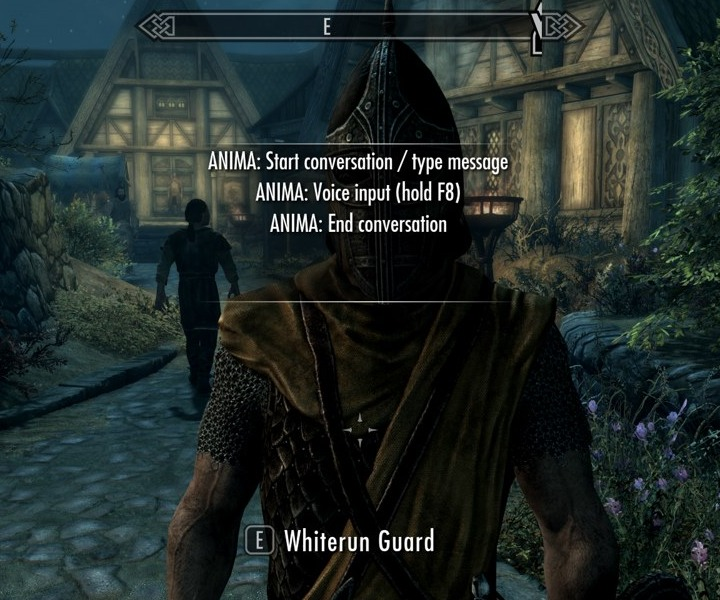
\includegraphics[width=.72\columnwidth]{figures/game_controls.jpg}
\caption{Anima conversation controls on a Whiterun Guard in Skyrim (native screenshot, cropped).}
\label{fig:game}
\end{figure}

\subsection{Computer Vision (RQ5)}
Table~\ref{tab:cv} consolidates the vision results. Half of the 128 pairs used one fixed adversarial descriptor with an override command, a false identity, a false attack and a fake quest marker. Among the 66 pairs that reached a prompt, nothing changed in the orchestration decisions and the adversarial text stayed in the untrusted block. Scripted models ignore the prompt, so whether a real model obeys adversarial on-screen text is unknown.

\begin{table}[t]
\caption{Computer-vision results. Language and vision models were scripted in the boundary tests. Inference rows come from small smoke tests.}
\label{tab:cv}
\centering\footnotesize\setlength{\tabcolsep}{3pt}
\begin{tabular}{>{\raggedright\arraybackslash}p{.6\columnwidth}>{\raggedright\arraybackslash}p{.32\columnwidth}}
\toprule
Measure & Result \\
\midrule
Paired turns; pairs reaching a prompt & 128; 66 \\
Plan, status, calls or evidence changed & 0 \\
Adversarial text outside untrusted block & 0 \\
Reply citing the camera frame & Refused \\
Prompt bytes added, one benign descriptor & 571 \\
Reply using a name only in the descriptor & Accepted (leak) \\
Frames 90\% near-black, original capture & 99 of 100 \\
Distinct frames 98\% black, original capture & 12 of 13 \\
Black share, revised capture ($n=5$) & 6.2\% \\
Capture time, revised, median ($n=5$) & 156 ms \\
Pipeline work excluding inference, median & 8.4--123.8 ms \\
Inference, first prompt: warm ($n=6$); cold & 3.4--6.0 s; 9.3 s \\
Inference, revised prompt: warm ($n=5$); cold & 3.3--5.0 s; 10.0 s \\
Black frame sent to first service & Invented scene \\
Detection, scene accuracy, dialogue benefit & Not measured \\
Frame time, GPU use, VRAM & Not measured \\
\bottomrule
\end{tabular}
\end{table}

The name check is a real leak. It accepts words from the descriptor, so a reply naming a person seen only on screen was rejected without the descriptor and accepted with it. Text in a frame can widen this check, though not any decision or knowledge binding.

The capture audit was the main practical finding. The original method's retained frames were almost entirely black, measured as luma below 8; they are retained frames, not a random sample. The cause was \texttt{BitBlt} on the window device context, which returned no pixels from this DirectX window, and fullscreen mode was not involved. \texttt{PrintWindow} with full-content rendering fixed this on the live game, though that test bypassed the foreground check and did not measure gameplay load. The first service described a figure and an object in an underground chamber for a black frame, so the service now rejects frames that are at least 98\% near-black.

Cold inference exceeds the 8~s wait inside a turn, so a cold result would be discarded. The revised prompt also filled the environment description, which was null on both public samples before. The live frame's description looked plausible by eye, naming a guard, torch and barrels, but this is no accuracy result. Vision has not yet run in a live conversation, so it has shown no benefit for dialogue, and it stays off by default.

\subsection{Discussion}
Binding decides what enters the prompt, and validation decides what leaves the layer, but neither controls what a model adds from its own weights. The observed details and related work~\cite{sadeq2024,ahn2024} show that knowledge binding and claim checking are complementary. Deterministic rules are repeatable and cheap, yet they leave most reworded hostility to the model.

\textit{Threats to validity.} We wrote the rules, labels, fictional worlds and expected outcomes, and the reply audit was AI-coded. One model and one game were used, and S3 predates the director. Live samples are small and span several builds; voices in the test setup came from a local Mantella folder, and voice-model licensing was not reviewed. No baseline against an unorchestrated model or Mantella exists, no human has rated believability, and no frame-time or VRAM result exists.

\section{Conclusion and Future Work}
Our orchestration layer decides how an NPC behaves and what it may know before any model is called, without training a model per game. Binding removed restricted facts from lower-standing prompts in two worlds, and a hosted model kept a peasant ignorant of the king's plan while able to pass on a rumour. The layer matched its rules and delivered no invalid reply under injected faults. In Skyrim, replies now complete and persist in memory, though one third of generated turns fell back and latency misses its targets. The design is intended to be reusable, but a second game remains untested.

Next steps are claim checking for unsupported details; a held-out, blinded human study comparing the director with a baseline and with an unorchestrated model; live retrieval with layered knowledge sources; and faster, more reliable live inference. For vision, the revised capture must be evaluated under gameplay load, and accuracy measured on labelled scenes before a live trial. A second connector will test generality directly.

\section*{Acknowledgment}
AI assistants were used for code, the dialogue audit and drafting; the authors are responsible for checking the content. Source, data and raw results: https://github.com/mohanchandrass/NPC.

\bibliographystyle{IEEEtran}
\bibliography{references}
\end{document}
